\documentclass[a4paper,oneside]{book}
\usepackage{geometry}
 \geometry{
 a4paper,
 total={170mm,257mm},
 left=20mm,
 top=20mm,
 }
\usepackage{pgfplots}
\pgfplotsset{width=7cm, compat=1.18}
\usepackage{indentfirst}
\usepackage{graphicx}
\graphicspath{ {./src/} }
\usepackage{hyperref}
\hypersetup{
    colorlinks=true,
    linkcolor=blue,
    filecolor=magenta,
    urlcolor=cyan,
}
\usepackage{longtable}
\usepackage{hhline}
\usepackage{booktabs}
\usepackage{makecell}
\usepackage{multirow}
\usepackage{array}
\usepackage{ragged2e}
\newcolumntype{R}[1]{>{\RaggedLeft\arraybackslash}p{#1}}
\newcommand\VRule[1][\arrayrulewidth]{\vrule width #1}
\usepackage[linesnumbered, boxed, ruled]{algorithm2e}
%% This declares a command \Comment
%% The argument will be surrounded by /* ... */
\SetKwComment{Comment}{/* }{ */}
\usepackage{tikz}
\usetikzlibrary{shapes.geometric, arrows}
%define boxes: startstop, io, process, decision, arrow
\tikzstyle{startstop} = [rectangle, rounded corners, minimum width=3cm, minimum height=1cm,text centered, draw=black, fill=red!30]
\tikzstyle{io} = [trapezium, trapezium left angle=70, trapezium right angle=110, minimum width=1cm, minimum height=1cm, text width=1cm, text centered, draw=black, fill=blue!30]
\tikzstyle{process} = [rectangle, minimum width=3cm, minimum height=1cm, text centered, draw=black, fill=orange!30]
\tikzstyle{decision} = [diamond, minimum width=3cm, minimum height=1cm, text centered, draw=black, fill=green!30]
\tikzstyle{arrow} = [thick,->,>=stealth]

\title{
    Maximum Submatrix Problem \\
    \large FDS Project1 Report}
\author{}
\date{\today}

\begin{document}

\clearpage
%% temporary titles
% command to provide stretchy vertical space in proportion
\newcommand\nbvspace[1][3]{\vspace*{\stretch{#1}}}
% allow some slack to avoid under/overfull boxes
\newcommand\nbstretchyspace{\spaceskip0.5em plus 0.25em minus 0.25em}
% To improve spacing on titlepages
\newcommand{\nbtitlestretch}{\spaceskip0.6em}
\pagestyle{empty}
\begin{center}
    \bfseries
    \nbvspace[1]
    \Huge
    {\nbtitlestretch\huge
        Maximum Submatrix Problem}

    \nbvspace[1]
    \normalsize

    Project 1 Report\\
    Fundamental of Data Structure (2023 Fall)\\
    Zhejiang University
    \nbvspace[1]
    \small BY\\
    \Large Baolin Zhu\\[0.5em]
    \footnotesize Student ID: 3220106026\\
    Teacher: HongHua Gan

    \nbvspace[2]
    Accomplished on October 3, 2023
    \nbvspace[3]
    \normalsize

    Made\\
    \large
    With \LaTeX
    \nbvspace[1]
\end{center}

\tableofcontents

\chapter{Introduction}

\section{Problem Description}

The Maximum Submatrix Sum Problem is a well-known problem in computer science
and mathematics. It can be formally defined as follows: given an $N \times M$
matrix $A$, we want to find the submatrix $B$ of maximal sum, where $B$ is a
contiguous rectangular subarray of $A$.

More specifically, we want to find $i_1, i_2, j_1, j_2$ such that $1 \leq i_1
    \leq i_2 \leq N$ and $1 \leq j_1 \leq j_2 \leq M$, and the sum of the elements
in the submatrix $B$ defined by rows $i_1$ through $i_2$ and columns $j_1$
through $j_2$ is maximized. In other words, we seek to maximize the quantity

\[\sum_{i = i_1}^{i_2} \sum_{j = j_1}^{j_2} A_{ij}\]

where $A_{ij}$ denotes the element in row $i$ and column $j$ of the matrix $A$.

\section{Problem Background}

The Maximum Submatrix Sum Problem is closely related to the Maximum Subsequence
Sum Problem we learned from class, but with some key differences. In the
Maximum Subsequence Sum Problem, we are given a sequence of numbers and we want
to find a subsequence with the maximum sum. This problem can be efficiently
solved using dynamic programming algorithms, such as Kadane's algorithm.

While Kadane's algorithm is not directly applicable to the Maximum Submatrix
Sum Problem due to the added dimensionality, it serves as an inspiration.
Various approaches and algorithms have been developed to tackle this problem
efficiently. One common approach is to transform the two-dimensional problem
into a one-dimensional problem by fixing one dimension and applying the maximum
subsequence sum algorithm. This technique, known as the ``2D Kadane's
algorithm'' or ``2D prefix sum'', can help identify the boundaries of the
optimal submatrix.

\chapter{Algorithm Specfication}

This chapter gives description of all the algorithms used for solving the
problem with specifications of main data structures.

\section{The Matrix Data Structure}

The \verb|Matrix| structure is simply a wrapper around an array of integers. It
contains the numbers of rows and columns of the matrix, as well as a pointer to
the array. I wrapped them in a structure for the convience of passing them
around as function arguments. It also simplifies the memory management, input
and output.

Here is the API of the \verb|Matrix| structure:

\begin{table}[!ht]
    \centering
    \caption{API of the \texttt{Matrix} structure}
    \begin{tabular}{R{0.1\textwidth} R{0.2\textwidth} p{0.2\textwidth} p{0.3\textwidth}}
        \toprule
        Type    & Name         & Arguments             & Description                \\
        \midrule
        Matrix* & CreateMatrix & (int rows, int cols)  & Create a matrix object     \\
        Matrix* & ReadMatrix   & (Matrix *m, File *fp) & Read matrix elements       \\
        void    & PrintMatrix  & (Matrix *m, File *fp) & Print matrix elements      \\
        void    & FreeMatrix   & (Matrix *m)           & Free matrix object         \\
        Matrix* & CopyMatrix   & (Matrix *m)           & Copy matrix object         \\
        Matrix* & MaxSubmatrix & (Matrix *m)           & Find the maximum submatrix \\
        \bottomrule
    \end{tabular}
\end{table}

\section{The First Algorithm}

This is the most straightforward algorithm. It simply tries all possible pairs
of rows and columns and computes the sum of the submatrix. It's pseudo-code is
displayed on the next page.

One thing need to be careful is that this algorithm (and the following two
algorithms) only works when there is at least one positive integer in the
matrix. This is because we initialize $maxSum$ to $0$, for there is no negative
infinity in C and we don't want to use \verb|INT_MIN| because it's not portable
and can cause overflow. The driver program will check if there is at least one
positive integer in the matrix before calling the algorithm.

\begin{algorithm}[H]
    \caption{The First Algorithm}\label{alg:1}
    \DontPrintSemicolon
    \KwIn{A matrix $A$ of size $N \times M$}
    \KwOut{The maximum submatrix $B$}
    \BlankLine
    $maxSum \gets 0$\;
    \For{$Left \gets 0$ \KwTo $M - 1$}{
        \For{$Right \gets maxLeft$ \KwTo $M - 1$}{
            \For{$Top \gets 0$ \KwTo $N - 1$}{
                \For{$Bottom \gets maxTop$ \KwTo $N - 1$}{
                    $sum \gets 0$\;
                    \For{$i \gets maxTop$ \KwTo $maxBottom$}{
                        \For{$j \gets maxLeft$ \KwTo $maxRight$}{
                            $sum \gets sum + A_{ij}$ \Comment*[r]{The main task}
                        }
                    }
                    \If{$sum > maxSum$}{
                        $maxSum \gets sum$\;
                        $maxLeft \gets Left$\;
                        $maxRight \gets Right$\;
                        $maxTop \gets Top$\;
                        $maxBottom \gets Bottom$\;
                    }
                }
            }
        }
    }
    \emph{Create and return the submatrix $B$}\;
\end{algorithm}

\section{The Second Algorithm}

We can improve the algorithm to avoid redundant computation. For example, when
the right bound of the submatrix increases, we would like to reuse the sum of
the left part of the submatrix.

In this algorithm, we use an temp array to store the sum of each row of the
submatrix. The maximum submatrix is then between the maximum subarray of the
temp array. As illustrated in~Figure~\ref{fig:alg2}:

\begin{figure}[!ht]
    \centering
    \caption{Illustration of the second algorithm}\label{fig:alg2}
    \includegraphics[width=0.5\textwidth]{alg2}
\end{figure}

\begin{algorithm}[H]
    \caption{The Second Algorithm}\label{alg:2}
    \DontPrintSemicolon
    \KwIn{A matrix $A$ of size $N \times M$}
    \KwOut{The maximum submatrix $B$}
    \BlankLine
    $maxSum \gets 0$\;
    \emph{Create an array $temp$ of size $N$}\;
    \For{$left \gets 0$ \KwTo $M - 1$}{
        \emph{Clean the array $temp$}\;
        \For{$right \gets left$ \KwTo $M - 1$}{
            \For{$i \gets 0$ \KwTo $N - 1$}{
                $temp[i] \gets temp[i] + A_{i, right}$ \Comment*[r]{Append new column}
            }
            \For{$i \gets 0$ \KwTo $N - 1$}{
                $sum \gets 0$\;
                \For{$j \gets i$ \KwTo $N - 1$}{
                    $sum \gets sum + temp[j]$ \Comment*[r]{The main task}
                    \If{$sum > maxSum$}{
                        $maxSum \gets sum$\;
                        $maxLeft \gets left$\;
                        $maxRight \gets right$\;
                        $maxTop \gets i$\;
                        $maxBottom \gets j$\;
                    }
                }
            }
        }
    }
    \emph{Create and return the submatrix $B$}\;
\end{algorithm}

\section{The Third Algorithm}

Noticing that the main task of the second algorithm is to find maximum subarray
of the temp array, we can use the Kadane's algorithm to improve that part of
the algorithm from $O(N^2)$ to $O(N)$.

\begin{algorithm}[H]
    \caption{The Third Algorithm}\label{alg:3}
    \DontPrintSemicolon
    \KwIn{A matrix $A$ of size $N \times M$}
    \KwOut{The maximum submatrix $B$}
    \BlankLine
    $maxSum \gets 0$\;
    \emph{Create an array $temp$ of size $N$}\;
    \For{$left \gets 0$ \KwTo $M - 1$}{
        \emph{Clean the array $temp$}\;
        \For{$right \gets left$ \KwTo $M - 1$}{
            \For{$i \gets 0$ \KwTo $N - 1$}{
                $temp[i] \gets temp[i] + A_{i, right}$\;
            }
            $sum \gets 0$\;
            $top \gets 0$\;
            \For{$i \gets 0$ \KwTo $N - 1$}{
                $sum \gets sum + temp[i]$ \Comment*[r]{Kadane's algorithm}
                \If{$sum > maxSum$}{
                    $maxSum \gets sum$\;
                    $maxTop \gets top$\;
                    $maxBottom \gets i$\;
                    $maxLeft \gets left$\;
                    $maxRight \gets right$\;
                }
                \If{$sum < 0$}{
                    $sum \gets 0$\;
                    $top \gets i + 1$\;
                }
            }
        }
    }
    \emph{Create and return the submatrix $B$}\;
\end{algorithm}

\section{Sketch of the Main Program}

The algorithm is just a library, so I wrote a driver program to run the
algorithm and generate the report. It will run the algorithm at least once and stop
when the total time is greater than 5 seconds.

\begin{figure}[!ht]
    \centering
    \caption{Sketch of the main program}
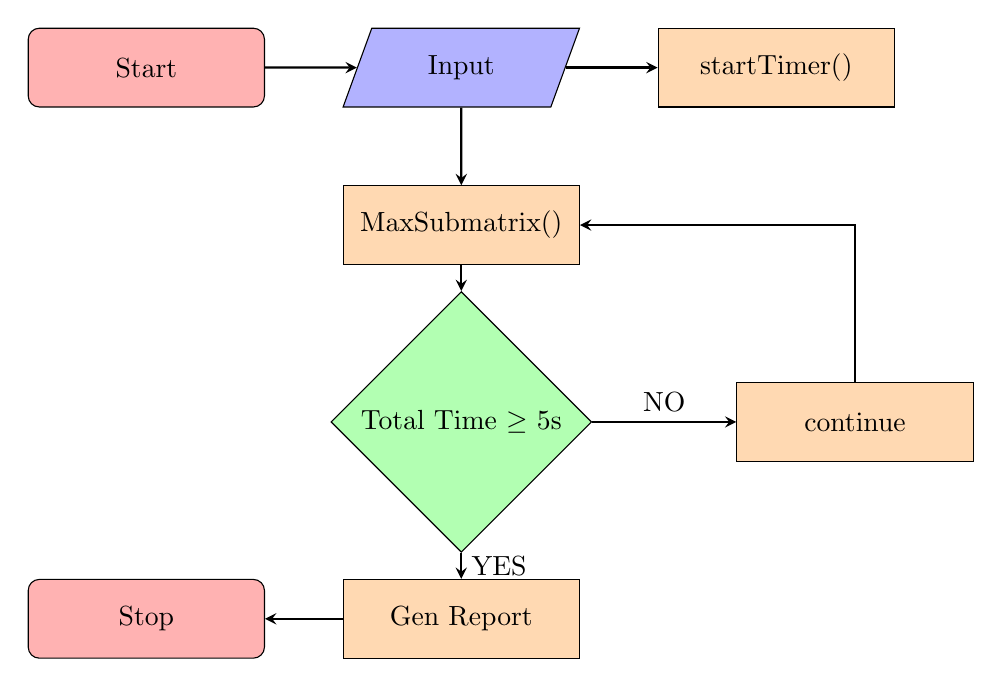
\begin{tikzpicture}[node distance=2cm]
    \node (start) [startstop] {Start};
    \node (input) [io, right of=start, xshift = 2cm] {Input};
    \node (timer) [process, right of=input, xshift = 2cm] {startTimer()};
    \node (max) [process, below of=input] {MaxSubmatrix()};
    \node (dec) [decision, below of=max, yshift=-0.5cm] {Total Time $\ge$ 5s};
    \node (print) [process, below of=dec, yshift=-0.5cm] {Gen Report};
    \node (continue) [process, right of=dec, xshift=3cm] {continue};
    \node (stop) [startstop, left of=print, xshift=-2cm] {Stop};
    \draw [arrow] (start) -- (input);
    \draw [arrow] (input) -- (timer);
    \draw [arrow] (input) -- (max);
    \draw [arrow] (max) -- (dec);
    \draw [arrow] (dec) -- node [anchor=south]{NO} (continue);
    \draw [arrow] (continue) |- (max);
    \draw [arrow] (dec) -- node [anchor=west]{YES} (print);
    \draw [arrow] (print) -- (stop);
\end{tikzpicture}
\end{figure}

\chapter{Testing Results}

\section{Test Data Generation}

I use \verb|rand()| to generate random integers in the range $[-100, 100]$ for
elements of the matrix. The size of the matrix is specified by the
teacher. For each size of the matrix, I generate five pieces of test data.

One thing to note is that there must be at least one positive integer in the
matrix. The minimum size of our test data is $5 \times 5$, and the probability
of having a test case with no positive integer is $0.5 ^ {25} \approx 2.3 \times
10^{-8}$. So we can safely ignore this case. The driver program will also check
if there is at least one positive integer in the input data. If not, it will
exit automatically.

\section{Testing Environment}

The program is compiled with \verb|clang 15| with target \verb|arm64-apple| and
\verb|-O3| flag on macOS Ventura. The CPU is \verb|Apple M2|. 

\section{Testing Results}

The test results here is the average value of five pieces of each group of test
data, so some statistics such as ticks may not be integers. But this makes the
results unaffected by the randomness of the test data.Raw test result is appended to the~Appendix~\ref{app:raw}. 

Here is the summary of the results:

\begin{table}[!ht]
    \centering
    \caption{Summary of the Results}\label{tab:summary}
    \begin{tabular}{||l|l||l|l|l|l|l|l||}
        \hhline{|t:==:t:======:t|}
                                              & N               & 5         & 10        & 30        & 50        & 80        & 100       \\
        \hhline{||==::======||}
        \multirow{4}{1.5cm}{$O(N^6)$ Version} & Iterations(K)   & 4036481   & 199315.8  & 639.4     & 40.8      & 3.8       & 1         \\
        \hhline{|~-||------|}                 & Ticks           & 5000000   & 5000012   & 5004622.6 & 5032313   & 6279354.8 & 5536404.6 \\
        \hhline{|~-||------|}                 & Total Time(sec) & 5         & 5.000012  & 5.0046226 & 5.032313  & 6.2793548 & 5.5364046 \\
        \hhline{|~-||------|}                 & Duration(sec)   & 1.24E-06  & 2.51E-05  & 7.83E-03  & 1.23E-01  & 1.65E+00  & 5.54E+00  \\
        \hhline{||==::======||}
        \multirow{4}{1.5cm}{$O(N^4)$ Version} & Iterations(K)   & 9876757.4 & 1487648.8 & 23522     & 3176.6    & 495.8     & 205.8     \\
        \hhline{|~-||------|}                 & Ticks           & 5000000.2 & 5000001.2 & 5000104   & 5000746.6 & 5006156   & 5010396.8 \\
        \hhline{|~-||------|}                 & Total Time(sec) & 5.0000002 & 5.0000012 & 5.000104  & 5.0007466 & 5.006156  & 5.0103968 \\
        \hhline{|~-||------|}                 & Duration(sec)   & 5.06E-07  & 3.36E-06  & 2.13E-04  & 1.57E-03  & 1.01E-02  & 2.43E-02  \\
        \hhline{||==::======||}
        \multirow{4}{1.5cm}{O($N^3)$ Version} & Iterations(K)   & 12877442  & 5894159   & 360422.4  & 62393.4   & 13770.8   & 7240.2    \\
        \hhline{|~-||------|}                 & Ticks           & 5000000.2 & 5000000   & 5000009.6 & 5000026.8 & 5000121.8 & 5000343.2 \\
        \hhline{|~-||------|}                 & Total Time(sec) & 5.0000002 & 5         & 5.0000096 & 5.0000268 & 5.0001218 & 5.0003432 \\
        \hhline{|~-||------|}                 & Duration(sec)   & 3.88E-07  & 8.48E-07  & 1.39E-05  & 8.01E-05  & 3.63E-04  & 6.91E-04  \\
        \hhline{|b:==:b:======:b|}
    \end{tabular}
\end{table}

From the table we can see: when $N$ doubles, the duration of the first algorithm
increases nearly $64$ times\footnote{Because the test data size is small, you
may not see the polynomial growth in the first few groups of data. But when $N$
gets larger, the polynomial growth becomes obvious. }, the duration of the
second algorithm increases nearly $16$ times and the duration of the third
algorithm increases nearly $8$ times. So we can guess that the time complexity
of the first algorithm is $O(N^6)$, of the second algorithm is $O(N^4)$ and of
the third algorithm is $O(N^3)$. In the next chapter, let's plot the data and
proof if our guess is correct.

\chapter{Analysis and Comments}

In this chapter, I will plot and proof the time and space complexity of the
three algorithms.

\section{Time Complexity}

\subsection{Line Chart of the Duration}

As you can see, there is huge performance difference between the three
when $N$ is large. The line chart of the first algorithm increases so fast
that the other two lines are almost horizontal. So I use a log scale for the
$y$ axis in the line chart below:

\begin{figure}[!ht]
    \caption{Duration of the Algorithms}\label{fig:duration}
    \centering
    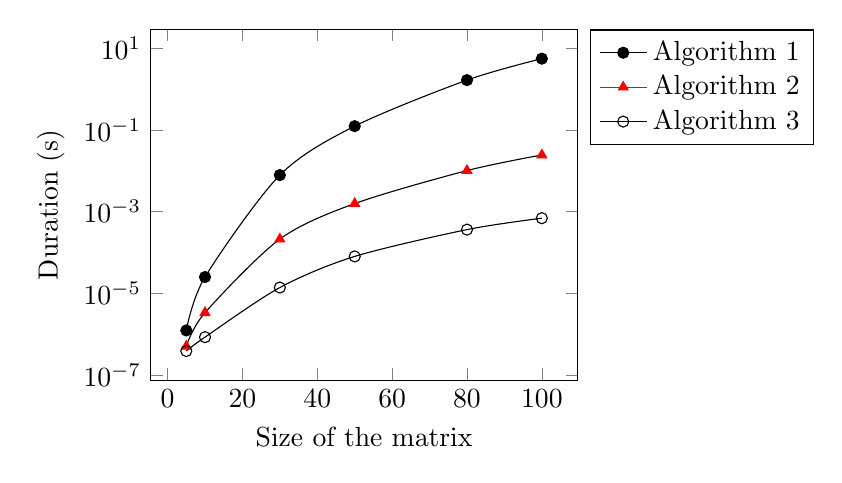
\begin{tikzpicture}
        \begin{axis}[
                %title={Duration of the Algorithms},
                ymode=log,
                log basis y={10},
                % log ticks with fixed point,
                xlabel={Size of the matrix},
                ylabel={Duration (s)},
                legend pos=outer north east
            ]
            \addplot [
                scatter,
                smooth,
                scatter src=explicit symbolic,
                scatter/classes={
                        1={black}
                    },
            ] table  {
                    x      y        label
                    5	0.0000012387027215 	1
                    10	0.0000250858787913  1
                    30	0.0078270606818893 	1
                    50	0.1233410049019610 	1
                    80	1.6524617894736800 	1
                    100	5.5364046000000000 	1
                };
            \addplot [
                scatter,
                smooth,
                scatter src=explicit symbolic,
                scatter/classes={
                        2={mark=triangle*,red}
                    },
            ] table [meta=label] {
                    x      y        label
                    5	0.0000005062390416 	2
                    10	0.0000033610091306 	2
                    30	0.0002125713799847 	2
                    50	0.0015742449789083 	2
                    80	0.0100971278741428 	2
                    100	0.0243459514091351 	2
                };
            \addplot [
                scatter,
                smooth,
                scatter src=explicit symbolic,
                scatter/classes={
                        3={mark=o,draw=black}
                    },
            ] table [meta=label] {
                    x      y        label
                    5	0.0000003882758858 	3
                    10	0.0000008482974416 	3
                    30	0.0000138726383266 	3
                    50	0.0000801371106559 	3
                    80	0.0003630959566619 	3
                    100	0.0006906360597774 	3
                };
            \legend{Algorithm 1, Algorithm 2, Algorithm 3}
        \end{axis}
    \end{tikzpicture}
\end{figure}

From the chart we can see that the time complexity of these algorithms are
polynomial. Using Excel, I linearly fitted the data after taking the logarithm,
and the results are displayed in the table below:

\begin{table}[!ht]
    \centering
    \caption{Regression Results}\label{tab:regression}
    \begin{tabular}{clc}
        \toprule
        Algorithm & Regression Equation & $R^2$ \\
        \midrule
        1         & $\log_{10}t=0.066N-5.1196$      & 0.8958 \\
        2         & $\log_{10}t=0.047N-5.7965$       & 0.9022 \\
        3         & $\log_{10}t=0.0342N-6.2408$       & 0.9364 \\
        \bottomrule
    \end{tabular}
\end{table}

Take care of the argument of $N$. They are related to the power exponent of the
complexity polynomial. We can easily guess there are multiple relations between
them. The arguments approximate the time complexity of the algorithms. This
discovery convinced me that our guess is correct. Proof of the time complexity
is in the following subsection.

\subsection{The First Algorithm}

As described in the~Algorithm~\ref{alg:1}, the main task is to compute the sum
of the submatrix. Line 9 is an $O(1)$ statement buried inside six nested
\verb|for| loops. All the loop size could be $N$, we must assume the worst case.
So the time complexity is $O(N^6)$.

\subsection{The Second Algorithm}

We used prefix sum to improve the first algorithm, so the main task is now find
maximum subarray of the temp array. Line 12 of~Algorithm~\ref{alg:2} is the main
task, and it's inside four nested \verb|for| loops, each can be $N$. So the time
complexity is $O(N^4)$.

\subsection{The Third Algorithm}

We used Kadane's algorithm to improve the second algorithm. Remember that we
proved that the time complexity of Kadane's algorithm is $O(N)$ in class. So the
time complexity of the third algorithm is $O(N^3)$. See line 12
of~Algorithm~\ref{alg:3}.

\subsection{Conclusion}

The analysis above proved that the time complexity of the first algorithm is
$O(N^6)$, of the second algorithm is $O(N^4)$ and of the third algorithm is
$O(N^3)$. $O(N^6) > O(N^4) > O(N^3)$, so the third algorithm is the fastest. We
can see each algorithm is faster than the previous one because reusing the
result of the previous step can save a lot of time. This is the main idea of
dynamic programming.

\section{Space Complexity}

In~Algorithm~\ref{alg:1}, we only need to store the $maxSum$, and the number of
other variables don't change with the size of the matrix. So the space
complexity is $O(1)$.

When it comes to~Algorithm~\ref{alg:2}, we need to store the temp array. The
size of the array is $N$, so the space complexity is $O(N)$. The same goes for
Algorithm~\ref{alg:3}.

So conclusions are here: the space complexity of the first algorithm is $O(1)$,
of the second and the third algorithm is $O(N)$. As illustrated in the chart
below:

\begin{figure}[!ht]
    \caption{Space Complexity of the Algorithms}\label{fig:space}
    \centering
    \includegraphics{src/space}
\end{figure}


\appendix

\chapter{Source Code}

The source code is in the \verb|code| directory. I've commented the source code
using Doxygen-style comments and generated the documentation file using Doxygen.
Please refer to the documentation file \href{run:./doxygen.pdf}{documents/doxygen.pdf} for
detailed comments.

\begin{enumerate}
    \item \verb|gen.c|: Test data generator.
    \item \verb|main.c|: Driver program.
    \item \verb|mss.h, mss.c|: Implementation of the algorithms.
\end{enumerate}

And here is the statistics of the source code above using \verb|cloc| tool:

\begin{verbatim}
-------------------------------------------------------------------------------
Language                     files          blank        comment           code
-------------------------------------------------------------------------------
C                                3             21            191            326
C/C++ Header                     1              9             63             18
-------------------------------------------------------------------------------
SUM:                             4             30            254            344
-------------------------------------------------------------------------------
\end{verbatim}

$42\%$ of the source code is well documented with Doxygen-style comments. This
satisfies the requirement of the project.


\chapter{User Manual}

\section{Makefile}

There are five targets in the \verb|code/Makefile|:

\begin{enumerate}
    \item \verb|all|: Run the target \verb|clean|, \verb|gen_data| and \verb|run|.
    \item \verb|gen_data|: For each of the size of N, generate five pieces of test data.
          The test data will be in \verb|data/| directory.
    \item \verb|mss|: Compile the driver program.
    \item \verb|run|: Compile and run the program through the test data and generate the report.
          Difference between each algorithms' result will be displayed using \verb|diff3|.
    \item \verb|clean|: Clean the generated files and data files.
\end{enumerate}

\section{Driver Program}
\label{app:driver}

The algorithm is just a library with no \verb|main()| function.
So I wrote a driver program to run the algorithm and generate the report.

The driver program is \verb|mss|. It takes two or three arguments:

\begin{enumerate}
\item \verb|data_file|: The file containing the matrix data.
\item \verb|algorithm|: The algorithm to use. It can be \verb|1|, \verb|2| or \verb|3|.
\item \verb|iteration|: If not specified, it will run the algorithm at least once and stop
when the total time is greater than 5 seconds.
\end{enumerate}

Usage:

\begin{verbatim}
    ./mss data_file algorithm [iteration]
\end{verbatim}

\chapter{Raw Test Results}\label{app:raw}

\begin{longtable}[c]{|l|l|r|l|l|l|}
    \caption{Raw Test Results}\label{long}                             \\
    \hline
    \multicolumn{6}{| c |}{Begin of Table}                             \\
    \hline
    Datasize & Algorithm & Iteration & Ticks   & Total Time & Duration \\
    \hline
    \endfirsthead

    \hline
    \multicolumn{6}{|c|}{Continuation of Table~\ref{long}}             \\
    \hline
    Datasize & Algorithm & Iteration & Ticks   & Total Time & Duration \\
    \hline
    \endhead

    \hline
    \endfoot

    \hline
    \multicolumn{6}{| c |}{End of Table}                               \\
    \hline\hline
    \endlastfoot

    100      & 1         & 1         & 5660987 & 5.660987   & 5.660987 \\
    100      & 2         & 202       & 5018513 & 5.018513   & 0.024844 \\
    100      & 3         & 7457      & 5000378 & 5.000378   & 0.000671 \\
    100      & 1         & 1         & 5534567 & 5.534567   & 5.534567 \\
    100      & 2         & 206       & 5005830 & 5.005830   & 0.024300 \\
    100      & 3         & 6822      & 5000405 & 5.000405   & 0.000733 \\
    100      & 1         & 1         & 5495957 & 5.495957   & 5.495957 \\
    100      & 2         & 207       & 5006043 & 5.006043   & 0.024184 \\
    100      & 3         & 8273      & 5000112 & 5.000112   & 0.000604 \\
    100      & 1         & 1         & 5494865 & 5.494865   & 5.494865 \\
    100      & 2         & 207       & 5013220 & 5.013220   & 0.024218 \\
    100      & 3         & 6959      & 5000216 & 5.000216   & 0.000719 \\
    100      & 1         & 1         & 5495647 & 5.495647   & 5.495647 \\
    100      & 2         & 207       & 5008378 & 5.008378   & 0.024195 \\
    100      & 3         & 6690      & 5000605 & 5.000605   & 0.000747 \\
    10       & 1         & 199688    & 5000002 & 5.000002   & 0.000025 \\
    10       & 2         & 1477115   & 5000000 & 5.000000   & 0.000003 \\
    10       & 3         & 6144195   & 5000000 & 5.000000   & 0.000001 \\
    10       & 1         & 199721    & 5000018 & 5.000018   & 0.000025 \\
    10       & 2         & 1510290   & 5000001 & 5.000001   & 0.000003 \\
    10       & 3         & 5812301   & 5000000 & 5.000000   & 0.000001 \\
    10       & 1         & 199129    & 5000011 & 5.000011   & 0.000025 \\
    10       & 2         & 1479740   & 5000001 & 5.000001   & 0.000003 \\
    10       & 3         & 6144876   & 5000000 & 5.000000   & 0.000001 \\
    10       & 1         & 199303    & 5000025 & 5.000025   & 0.000025 \\
    10       & 2         & 1489116   & 5000002 & 5.000002   & 0.000003 \\
    10       & 3         & 5807918   & 5000000 & 5.000000   & 0.000001 \\
    10       & 1         & 198738    & 5000004 & 5.000004   & 0.000025 \\
    10       & 2         & 1481983   & 5000002 & 5.000002   & 0.000003 \\
    10       & 3         & 5561505   & 5000000 & 5.000000   & 0.000001 \\
    30       & 1         & 626       & 5000133 & 5.000133   & 0.007987 \\
    30       & 2         & 23578     & 5000169 & 5.000169   & 0.000212 \\
    30       & 3         & 357285    & 5000011 & 5.000011   & 0.000014 \\
    30       & 1         & 659       & 5006499 & 5.006499   & 0.007597 \\
    30       & 2         & 23794     & 5000086 & 5.000086   & 0.000210 \\
    30       & 3         & 359447    & 5000008 & 5.000008   & 0.000014 \\
    30       & 1         & 649       & 5003665 & 5.003665   & 0.007710 \\
    30       & 2         & 23553     & 5000075 & 5.000075   & 0.000212 \\
    30       & 3         & 348357    & 5000006 & 5.000006   & 0.000014 \\
    30       & 1         & 649       & 5006525 & 5.006525   & 0.007714 \\
    30       & 2         & 23690     & 5000142 & 5.000142   & 0.000211 \\
    30       & 3         & 356017    & 5000016 & 5.000016   & 0.000014 \\
    30       & 1         & 614       & 5006291 & 5.006291   & 0.008154 \\
    30       & 2         & 22995     & 5000048 & 5.000048   & 0.000217 \\
    30       & 3         & 381006    & 5000007 & 5.000007   & 0.000013 \\
    50       & 1         & 40        & 5023702 & 5.023702   & 0.125593 \\
    50       & 2         & 3182      & 5000975 & 5.000975   & 0.001572 \\
    50       & 3         & 63281     & 5000015 & 5.000015   & 0.000079 \\
    50       & 1         & 41        & 5034499 & 5.034499   & 0.122793 \\
    50       & 2         & 3181      & 5000700 & 5.000700   & 0.001572 \\
    50       & 3         & 60882     & 5000016 & 5.000016   & 0.000082 \\
    50       & 1         & 41        & 5007455 & 5.007455   & 0.122133 \\
    50       & 2         & 3193      & 5000249 & 5.000249   & 0.001566 \\
    50       & 3         & 61067     & 5000031 & 5.000031   & 0.000082 \\
    50       & 1         & 41        & 5050169 & 5.050169   & 0.123175 \\
    50       & 2         & 3164      & 5000810 & 5.000810   & 0.001581 \\
    50       & 3         & 68454     & 5000051 & 5.000051   & 0.000073 \\
    50       & 1         & 41        & 5045740 & 5.045740   & 0.123067 \\
    50       & 2         & 3163      & 5000999 & 5.000999   & 0.001581 \\
    50       & 3         & 58283     & 5000021 & 5.000021   & 0.000086 \\
    5        & 1         & 4082538   & 5000000 & 5.000000   & 0.000001 \\
    5        & 2         & 9479643   & 5000000 & 5.000000   & 0.000001 \\
    5        & 3         & 12471285  & 5000000 & 5.000000   & 0.000000 \\
    5        & 1         & 3988896   & 5000000 & 5.000000   & 0.000001 \\
    5        & 2         & 10117125  & 5000000 & 5.000000   & 0.000000 \\
    5        & 3         & 12946018  & 5000001 & 5.000001   & 0.000000 \\
    5        & 1         & 3973865   & 5000000 & 5.000000   & 0.000001 \\
    5        & 2         & 10122368  & 5000001 & 5.000001   & 0.000000 \\
    5        & 3         & 12902282  & 5000000 & 5.000000   & 0.000000 \\
    5        & 1         & 4080377   & 5000000 & 5.000000   & 0.000001 \\
    5        & 2         & 10128950  & 5000000 & 5.000000   & 0.000000 \\
    5        & 3         & 12776740  & 5000000 & 5.000000   & 0.000000 \\
    5        & 1         & 4056729   & 5000000 & 5.000000   & 0.000001 \\
    5        & 2         & 9535701   & 5000000 & 5.000000   & 0.000001 \\
    5        & 3         & 13290885  & 5000000 & 5.000000   & 0.000000 \\
    80       & 1         & 4         & 6605185 & 6.605185   & 1.651296 \\
    80       & 2         & 502       & 5010748 & 5.010748   & 0.009982 \\
    80       & 3         & 14016     & 5000022 & 5.000022   & 0.000357 \\
    80       & 1         & 4         & 6554565 & 6.554565   & 1.638641 \\
    80       & 2         & 497       & 5009081 & 5.009081   & 0.010079 \\
    80       & 3         & 12634     & 5000017 & 5.000017   & 0.000396 \\
    80       & 1         & 3         & 5002091 & 5.002091   & 1.667364 \\
    80       & 2         & 493       & 5004294 & 5.004294   & 0.010151 \\
    80       & 3         & 13625     & 5000312 & 5.000312   & 0.000367 \\
    80       & 1         & 4         & 6583925 & 6.583925   & 1.645981 \\
    80       & 2         & 491       & 5001074 & 5.001074   & 0.010185 \\
    80       & 3         & 14861     & 5000090 & 5.000090   & 0.000336 \\
    80       & 1         & 4         & 6651008 & 6.651008   & 1.662752 \\
    80       & 2         & 496       & 5005583 & 5.005583   & 0.010092 \\
    80       & 3         & 13718     & 5000168 & 5.000168   & 0.000364 \\
\end{longtable}

The diff results of three algorithms are as follows, the output is truncated:

\begin{verbatim}
for file in data/100_0.txt data/100_1.txt data/100_2.txt data/100_3.txt 
data/100_4.txt data/10_0.txt data/10_1.txt data/10_2.txt data/10_3.txt 
data/10_4.txt data/30_0.txt data/30_1.txt data/30_2.txt data/30_3.txt 
data/30_4.txt data/50_0.txt data/50_1.txt data/50_2.txt data/50_3.txt 
data/50_4.txt data/5_0.txt data/5_1.txt data/5_2.txt data/5_3.txt 
data/5_4.txt data/80_0.txt data/80_1.txt data/80_2.txt data/80_3.txt 
data/80_4.txt; do \
        echo "Running $file"; \
        ./mss $file 1 >> $file.1out; \
        ./mss $file 2 >> $file.2out; \
        ./mss $file 3 >> $file.3out; \
        diff3 $file.1out $file.2out $file.3out; \
    done
Running data/100_0.txt
====
1:2c
  algorithm: 1
2:2c
  algorithm: 2
3:2c
  algorithm: 3
Running data/100_1.txt
====
1:2c
  algorithm: 1
2:2c
  algorithm: 2
3:2c
  algorithm: 3
Running data/100_2.txt 
...
\end{verbatim}

All three algorithms output the same result matrix for each test case. Here is
one example of \verb|data/5_0.txt.1out|:

\begin{verbatim}
datafile: data/5_0.txt
algorithm: 1
MaxSubmatrix: 
44       -22      23       9        
65       -8       -58      87       
27       29       -60      -88      
69       9        57       60       
\end{verbatim}

\chapter{Declaration}

I hereby declare that all the work done in this project titled ``Maximum
Submatrix Problem'' is of my independent effort.

\end{document}